
%----------------------------------------------------------------------------------------
%	CHAPTER 2
%----------------------------------------------------------------------------------------

\chapter{\textcolor{blue}{\Footwork~(Footwork) em samba de gafieira}}

Uma parte muito importante do desenvolvimento na dança é o treino e a repetição;
nesse sentido, o dançarino muitas vesses tem que investir em se mesmo muito tempo 
de treinamento para desenvolver de forma fluida e natural seus movimentos.
Este é um trabalho duro e contínuo, que muitas vesses abordaremos de forma individual, 
no nosso próprio tempo de aprendizagem; 
por isso é importante conhecer uma serie de exercícios que nos preparem,
fisicamente, e nos deem consciência corporal para executar nossos movimentos na dança.

Nas seguintes seções serão apresentadas, uma serie de movimentos que podem ser usados,
no treinamento unipessoal, eles estão representados usando uma notação coreográfica
para o \footwork, que será previamente explicada.
 
\section{Notação coreográfica para o \footwork }
Para descrever o \footwork~ numa representação escrita, 
será usado uma notação baseada numa vista da posição dos pés no chão. 
Existirá uma representação para cada subdivisão temporal do movimento, 
estas subdivisões serão chamadas de tempos coreográficos, 
para diferenciar-lhos dos tempos do compasso; 
pois a duração e o inicio destos será diferente\footnote{Para 
mais detalhes da contagem dos tempos no compasso, ver Seção \ref{sec:Tempo}.}.

A Tabela \ref{tab:notationunipessoal} descreve o significado de todos os símbolos usados,
na notação coreográfica para o \footwork.
\begin{longtable}{| p{0.1\textwidth}|p{0.80\textwidth}  |}
  %\begin{tabular}{| p{0.1\textwidth}|p{0.80\textwidth}  |}
  \hline
  Símbolo & Descrição \\ \hline \hline 
  T & Abreviatura do termo \textbf{tempo}, se referindo ao tempo do compasso na música, ver Seção \ref{sec:Tempo}. \\ \hline

  TC & Abreviatura do termo \textbf{tempo coreográfico}, 
  de modo que cada movimento é subdividido temporalmente num número de TC. 
  Todos os TC são definidos na descrição de cada movimento, 
  tendo sempre neste âmbito a mesma duração;
  porem, este é um valor relativo ao tempo musical, e cada movimento pode usar um TC de 1, 1/2 ou 1/4 do tempo musical,
  procurando otimizar a didática na explicação do movimento. \\ \hline

  \raisebox{-\totalheight}{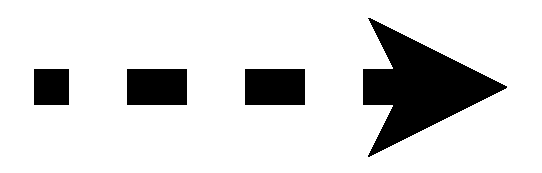
\includegraphics[width=1cm]{notation-foot/notacion1-seta.eps}} & A \textbf{seta} 
  indica o percorrido para que um pé chegue à posição do TC atual; é dizer, nos fala do passado do TC.
  A cor pode variar em função se no final do movimento se chega com o peso do corpo. \\ \hline 

  \raisebox{-\totalheight}{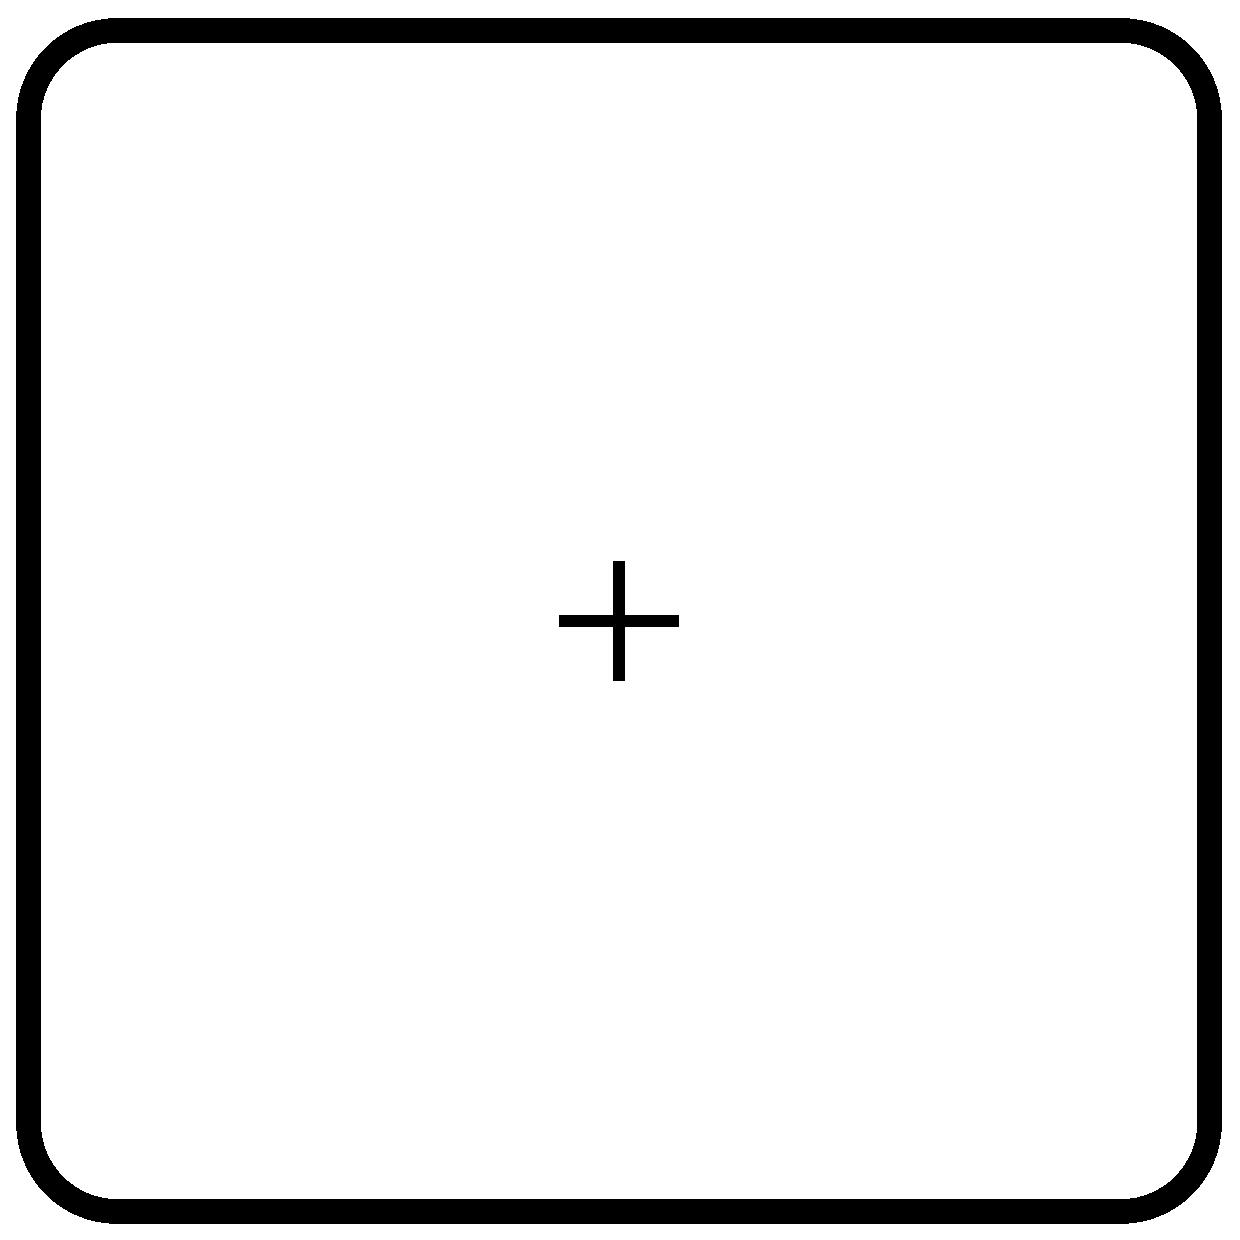
\includegraphics[width=1cm]{notation-foot/notacion-box.eps}} & 
  O \textbf{quadro de trabalho} é onde se colocará a disposição dos pés no chão, em cada tempo coreográfico,
  de modo que esta disposição indica o estado no inicio do TC.
  A posição onde o dançarino referencia seu \footwork~ é indicado com um símbolo de +.  \\ \hline

  \raisebox{-\totalheight}{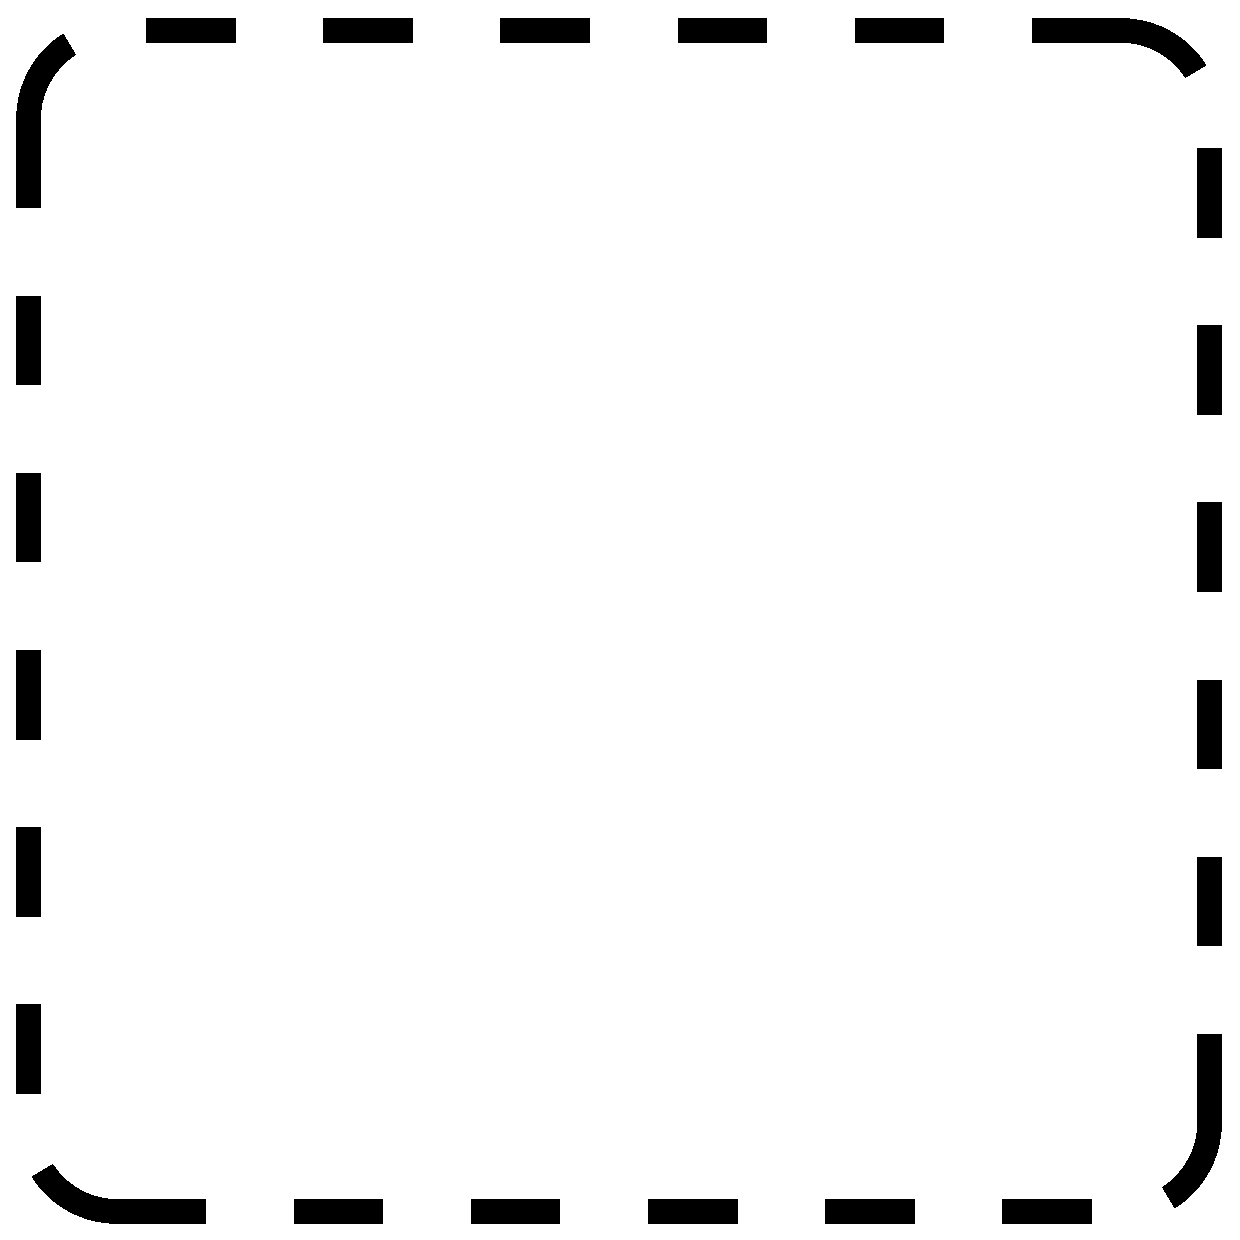
\includegraphics[width=1cm]{notation-foot/notacion-box-dot.eps}} & 
  O \textbf{quadro de descanso} é um símbolo que indica que nesse tempo coreográfico não se realizará movimento de pés,
  e se manterá a posição o TC anterior.  \\ \hline


  \raisebox{-\totalheight}{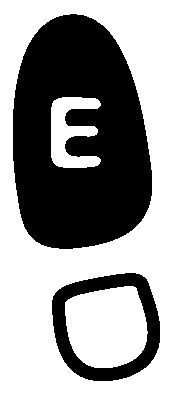
\includegraphics[height=1.0cm]{notation-foot/notacion-esq-preto.eps}} & Este símbolo 
  indica o \textbf{pé esquerdo}, a cor pode variar em função se este tiver o peso do corpo. \\ \hline  

  \raisebox{-\totalheight}{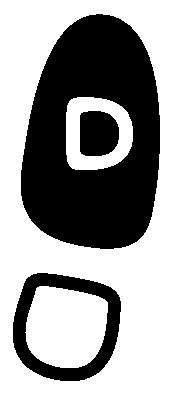
\includegraphics[height=1.00cm]{notation-foot/notacion-der-preto.eps}} & Este símbolo 
  indica o \textbf{pé direito}, a cor pode variar em função se este tiver o peso do corpo. \\ \hline

  \raisebox{-\totalheight}{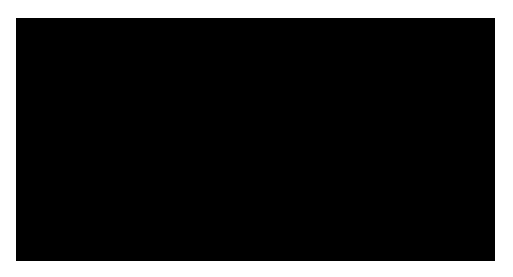
\includegraphics[width=1cm]{notation-foot/notacion-preto.eps}} & Os símbolos 
  com esta cor indicam que esse pé \textbf{tem o peso do corpo}. \\ \hline 

  \raisebox{-\totalheight}{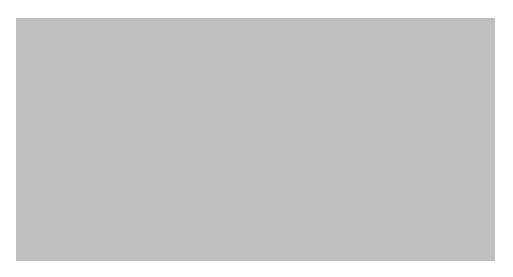
\includegraphics[width=1cm]{notation-foot/notacion-gris.eps}} & Os símbolos 
  com esta cor indicam que esse pé \textbf{não tem o peso do corpo}. \\ \hline

  %\end{tabular}
  \caption{Notação coreográfica para o \footwork.}
  \label{tab:notationunipessoal}
\end{longtable}

\section{\textcolor{blue}{Movimentos para trabalhar de forma individual}}

Nesta seção serão descritos uma serie de movimentos que poderão ser treinados individualmente.
Estes são interessantes para o desenvolvimento de consciência corporal, 
e poderão ser usados posteriormente na dança a dois,
fazendo algumas leves modificações ou adaptações.

\begin{tcbattention}
Nas seguintes subseções, é usado o termo \textbf{variante} para descrever aos movimentos;
devido a que para cada movimento, na dança, 
existe uma grande variedade de formas ou estilos de realizar estes.
Assim, é difícil estabelecer um critério comum para apontar a forma oficial para a realização de cada movimento,
pelo que estes serão referenciados sempre como variantes. 
\end{tcbattention}

\subsection{ \Variante: Trança}
\index{Passo!Trança}

A Figura \ref{fig:pessoaltranca} mostra uma variante do movimento chamado trança.
Cada quadro de trabalho representa a posição dos pés em cada tempo coreográfico;
um tempo coreográfico tem uma duração igual a meio tempo musical.
A trança é um movimento que pode ser executado de forma cíclica, de modo que 
a sequencia de passos pode executa-se como: TC1, TC2, ..., TC7, TC8, TC1, ..., etc.  
Quantas vesse o considere necessário.
\begin{figure}[h]
  \centering
    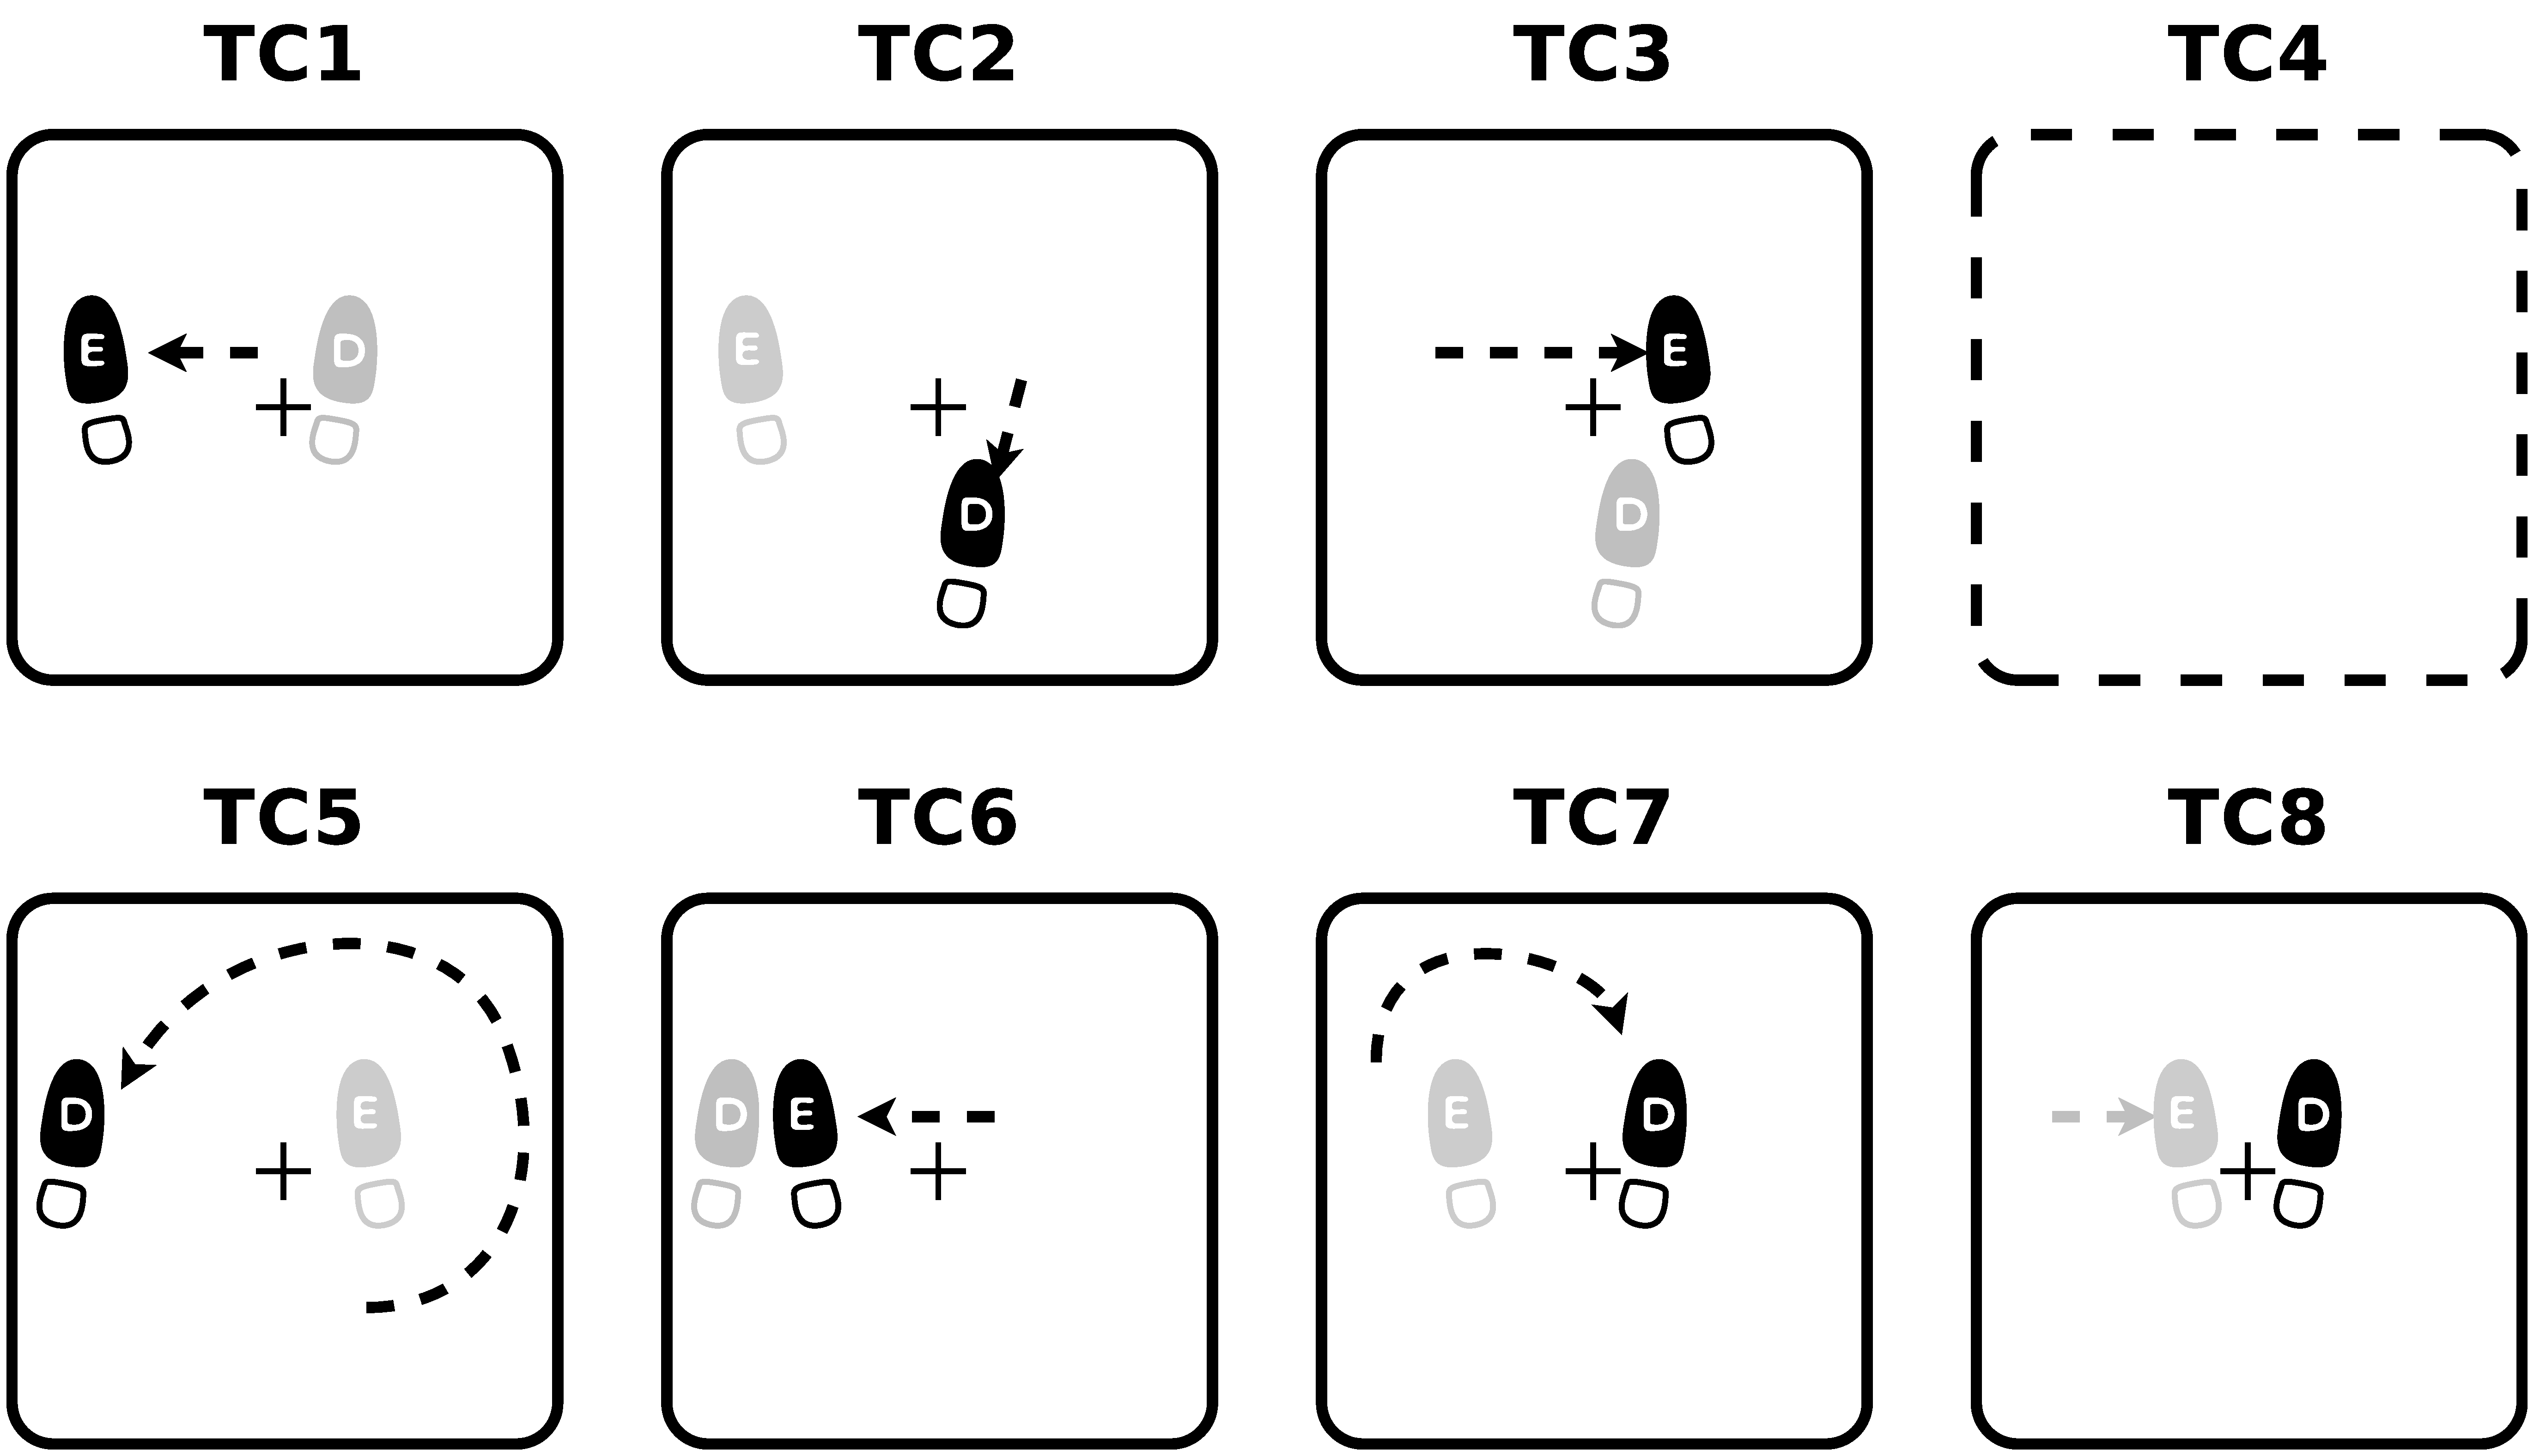
\includegraphics[width=0.75\textwidth]{chapters/cap-passos-footwork/tranca.eps}
\caption{Diagrama de tempos coreográficos para a trança, $T/2=TC$.}
\label{fig:pessoaltranca}
\end{figure}

A Figura \ref{fig:abc-pessoaltrancatc2} mostra o diagrama de tempos para realizar o movimento trança,
iniciando com o tempo forte da música.
\begin{figure}[h]
  \centering
\begin{abc}[name=abc-pessoaltrancatc2,width=0.6\linewidth]
X: 1 % start of header
K: C stafflines=1 % scale: C major
M: 2/4 %meter - compasso
%Q:1/4=80
V:1 clef=perc stem=up name="Ritmo" sname="Ritmo"
V:2 clef=perc stem=up name="TC"    sname="TC"
[V:1] |: B2  B1  B1 | B2  B1  B1 :| 
w:       tum  tchic tchic tum tchic tchic 
w: ~ ~ ~ ~ ~ ~ 
%w: ~ ~ ~ ~ ~ ~ 
[V:2] |: B1  B1  B1  B1 | B1 B1  B1  B1 :| 
w:       TC1 TC2  TC3 TC4 TC5 TC6 TC7 TC8
\end{abc}
\caption{Diagrama de tempos para a execução da trança.}
\label{fig:abc-pessoaltrancatc2}
\end{figure}

Dependendo do movimento ou passo, desde onde entremos na trança, 
em algumas momentos faremos este movimento iniciando desde o tempo fraco da música; 
nesse contexto, a Figura \ref{fig:abc-pessoaltranca} mostra a distribuição de tempos para realizar 
este movimento.
\begin{figure}[h]
  \centering
\begin{abc}[name=abc-pessoaltranca,width=0.6\linewidth]
X: 1 % start of header
K: C stafflines=1 % scale: C major
M: 2/4 %meter - compasso
%Q:1/4=80
V:1 clef=perc stem=up name="Ritmo" sname="Ritmo"
V:2 clef=perc stem=up name="TC"    sname="TC"
[V:1] |: B2  B1  B1 | B2  B1  B1 :| 
w:       ~   tchic tchic tum tchic tchic 
w:       tum ~     ~     ~   ~     ~    
w: ~ ~ ~ ~ ~ ~ 
%w: ~ ~ ~ ~ ~ ~ 
[V:2] |: B1  B1  B1  B1 | B1 B1  B1  B1 :| 
w:       ~   ~   TC1 TC2  TC3 TC4 TC5 TC6 
%w:       ~ ~ ~ ~   ~ ~ ~ ~ 
w:       TC7 TC8  ~  ~    ~   ~   ~   ~    
\end{abc}
\caption{Diagrama de tempos para a execução da trança.}
\label{fig:abc-pessoaltranca}
\end{figure}


\subsection{\textcolor{red}{\Variante: Samba no pé}}\index{Passo!Samba no pé}

A Figura \ref{fig:pessoa-samba-no-pe} mostra o diagrama de tempos para realizar o movimento.

\begin{figure}[h]
  \centering
    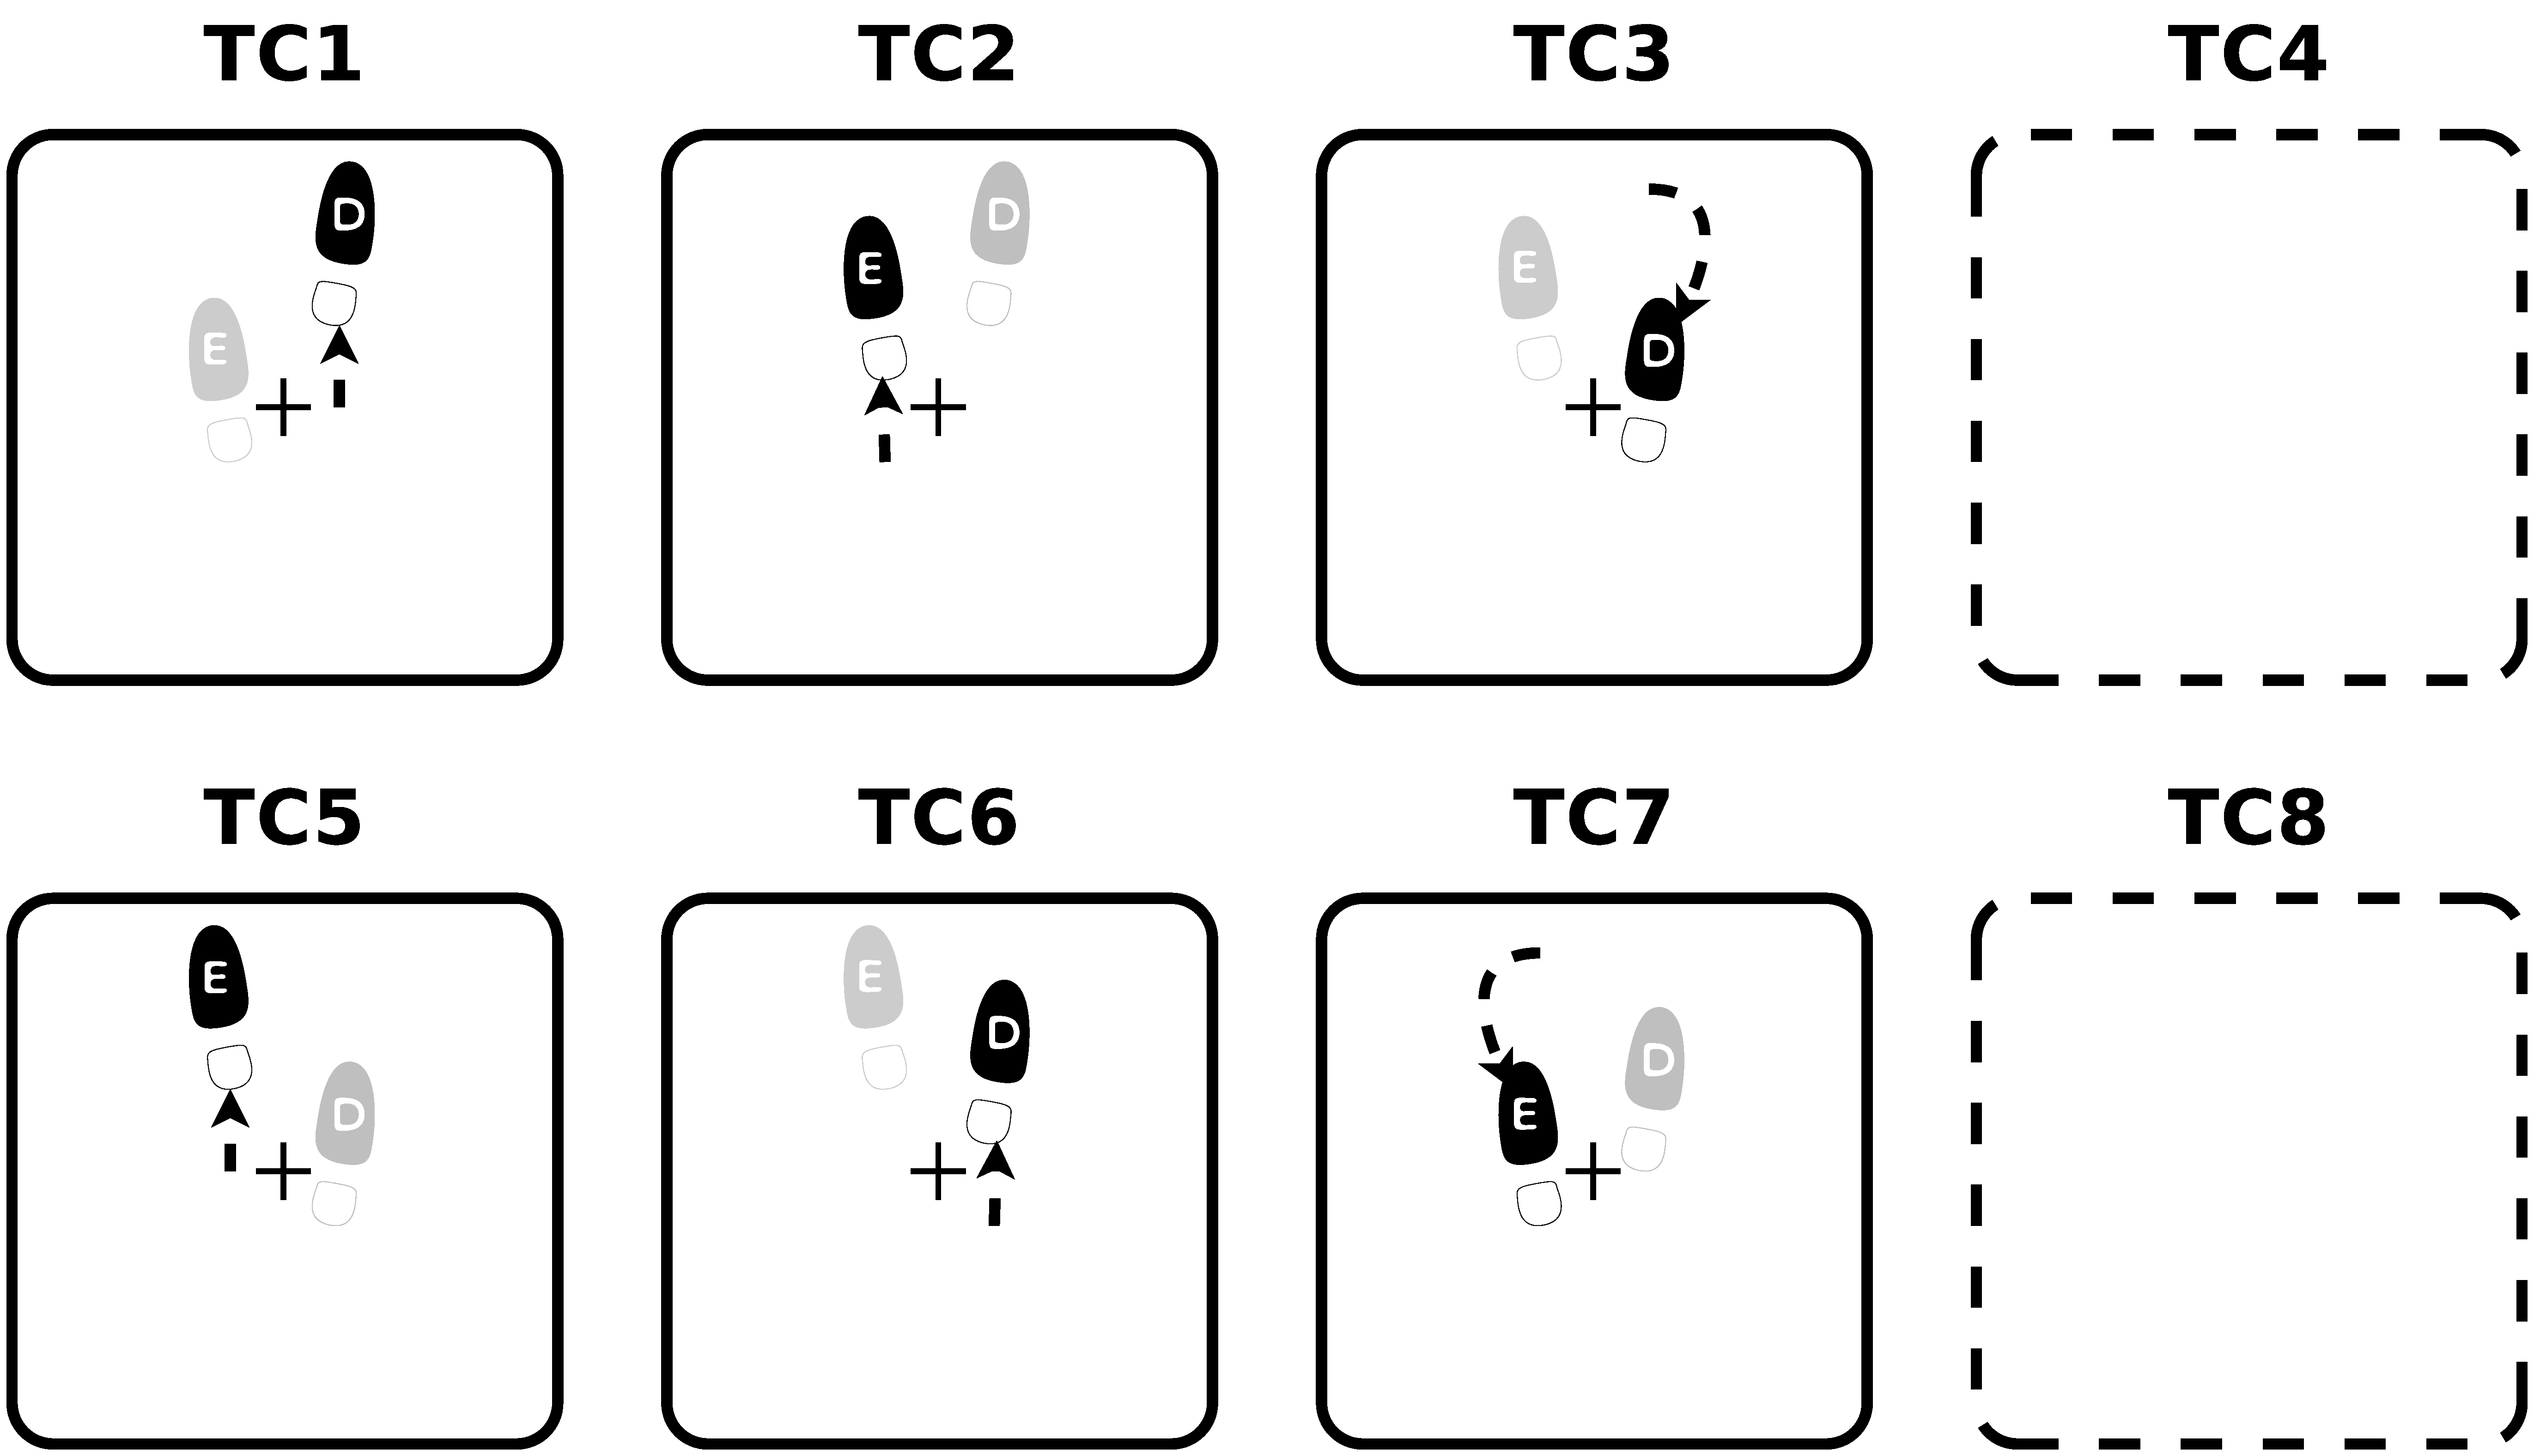
\includegraphics[width=0.75\textwidth]{chapters/cap-passos-footwork/samba-no-pe.eps}
\caption{Diagrama de tempos coreográficos para o passo de samba no pé, $T/2=TC$.}
\label{fig:pessoa-samba-no-pe}
\end{figure}

\subsection{\textcolor{red}{\Variante~2: Samba no pé}}\index{Passo!Samba no pé}

A Figura \ref{fig:pessoa-samba-no-pe-b} mostra o diagrama de tempos para realizar o movimento.

\begin{figure}[h]
  \centering
    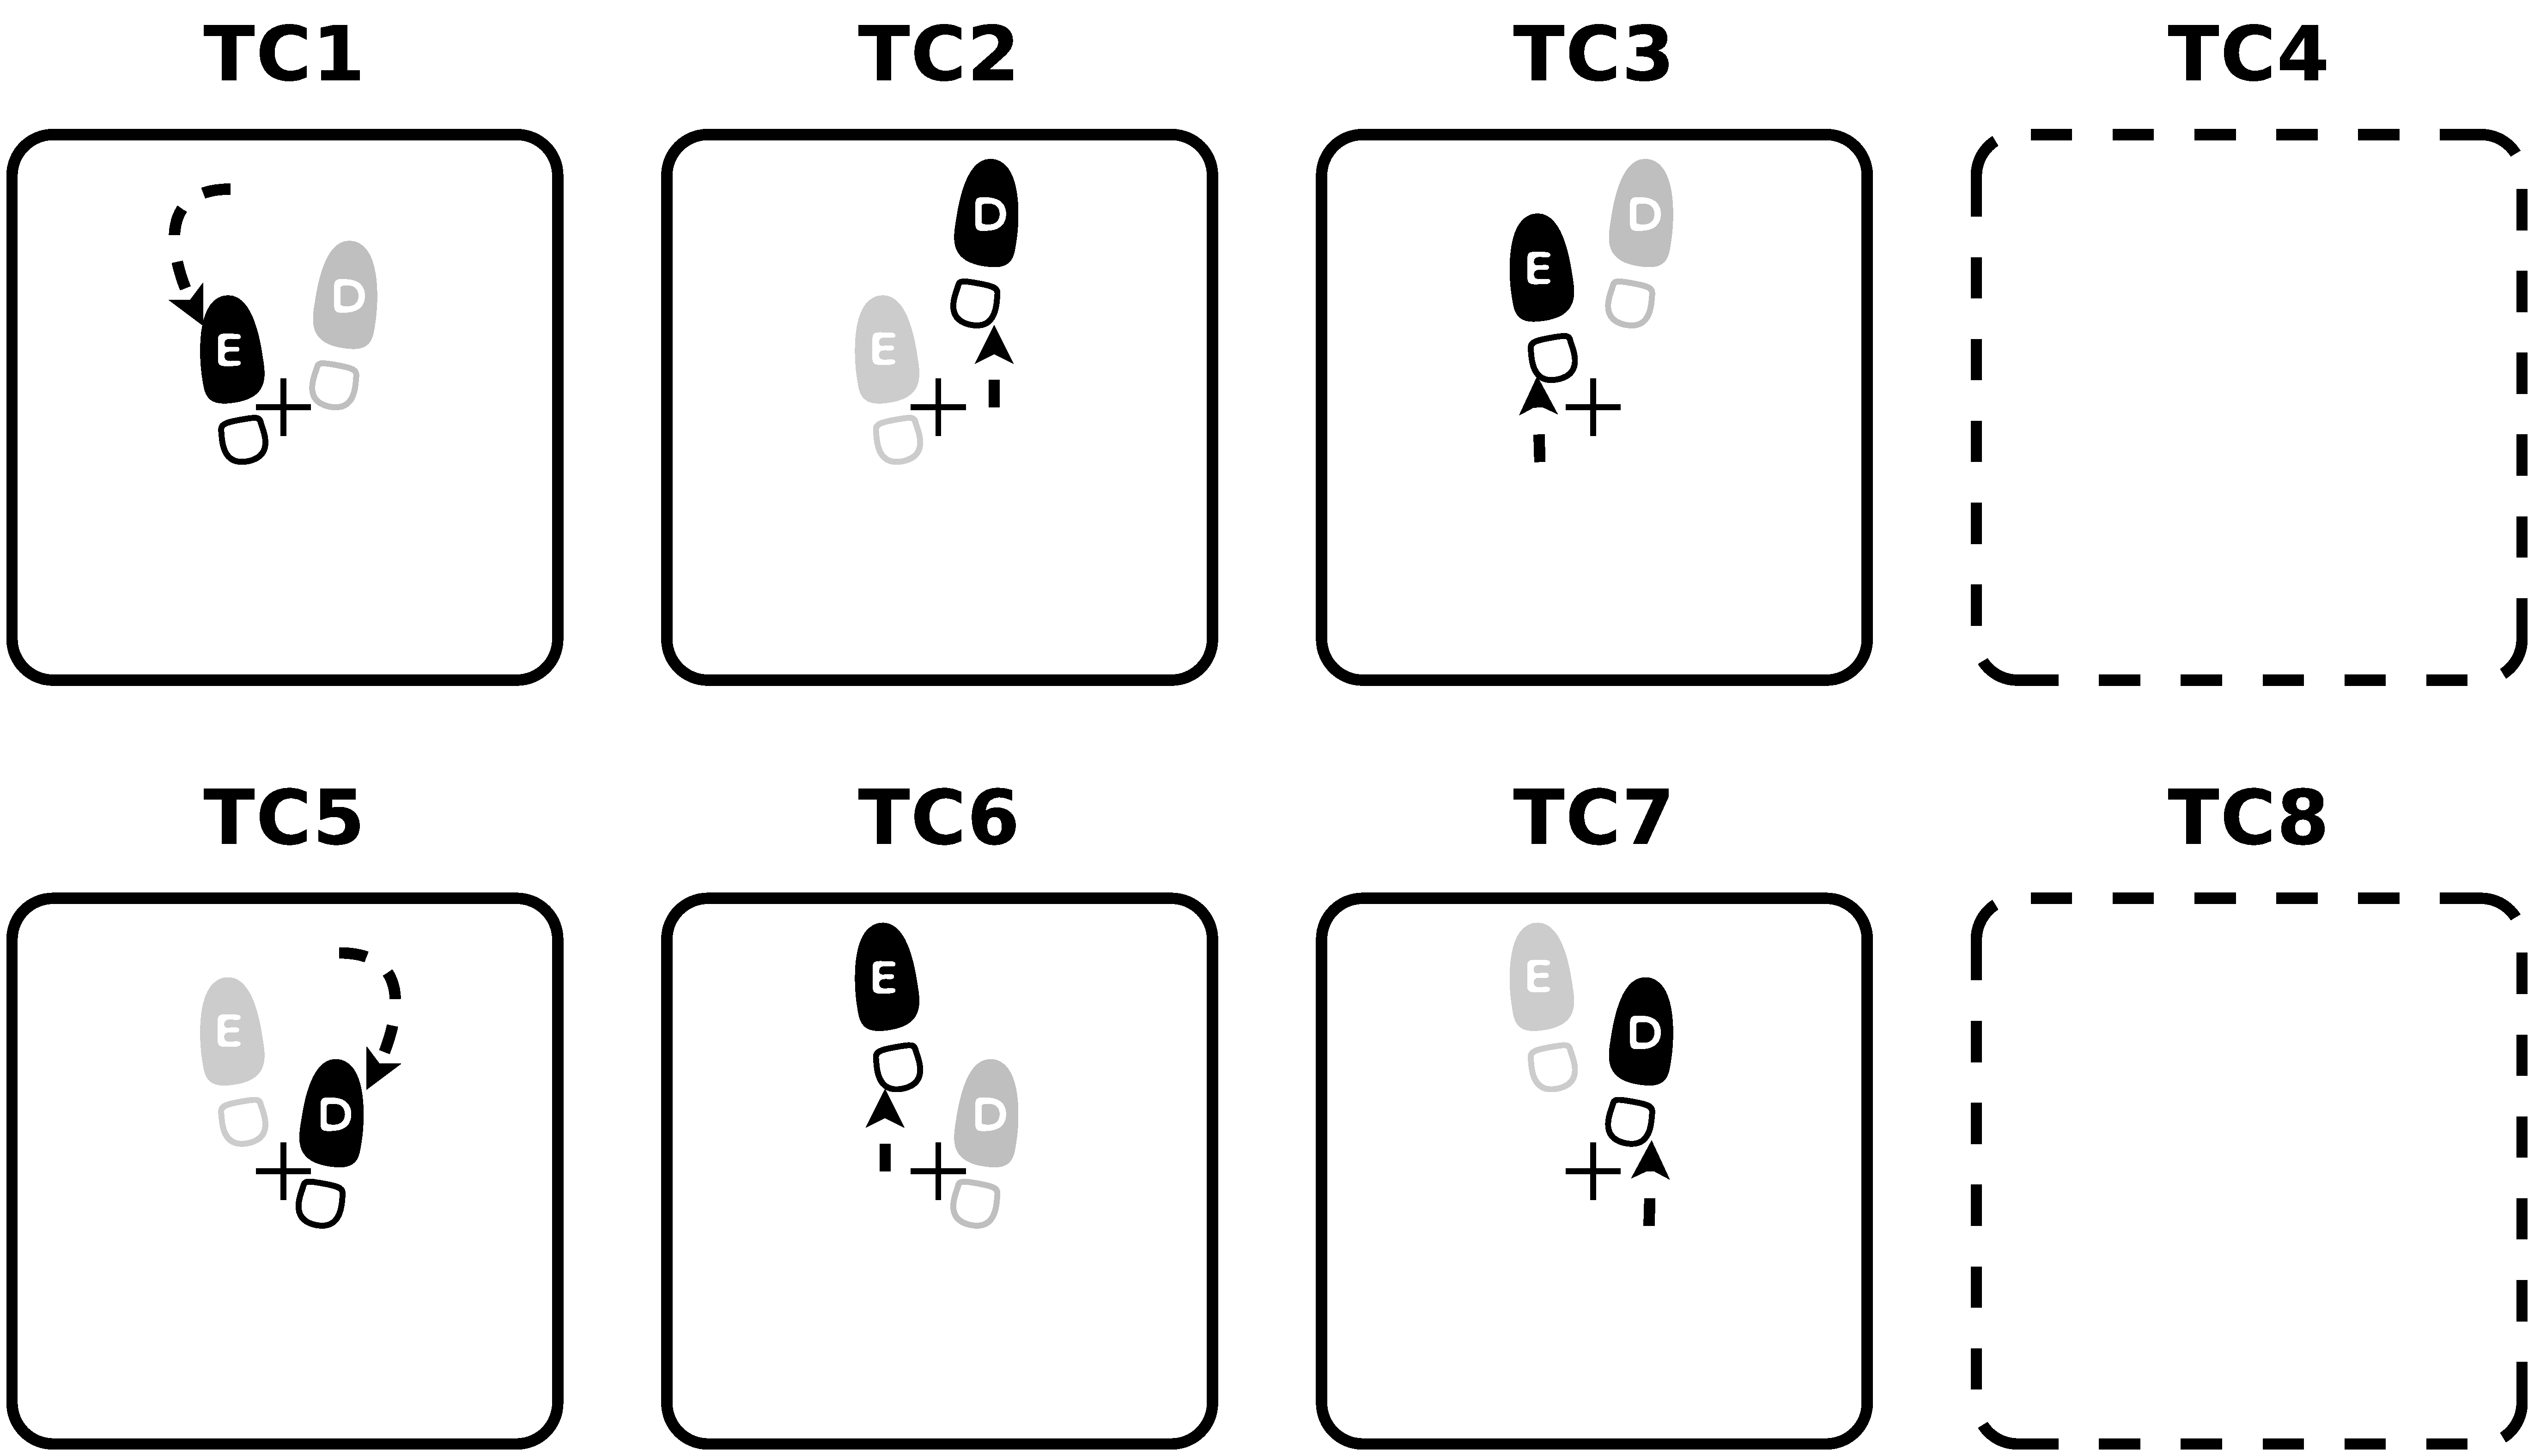
\includegraphics[width=0.75\textwidth]{chapters/cap-passos-footwork/samba-no-pe-b.eps}
\caption{Diagrama de tempos coreográficos para o passo de samba no pé, $T/2=TC$.}
\label{fig:pessoa-samba-no-pe-b}
\end{figure}

\subsection{\textcolor{red}{\Variante: Samba no pé (para adiante)}}\index{Passo!Samba no pé para adiante}
A Figura \ref{fig:pessoa-samba-no-pe-adiante} mostra o diagrama de tempos para realizar o movimento.

\begin{figure}[h]
  \centering
    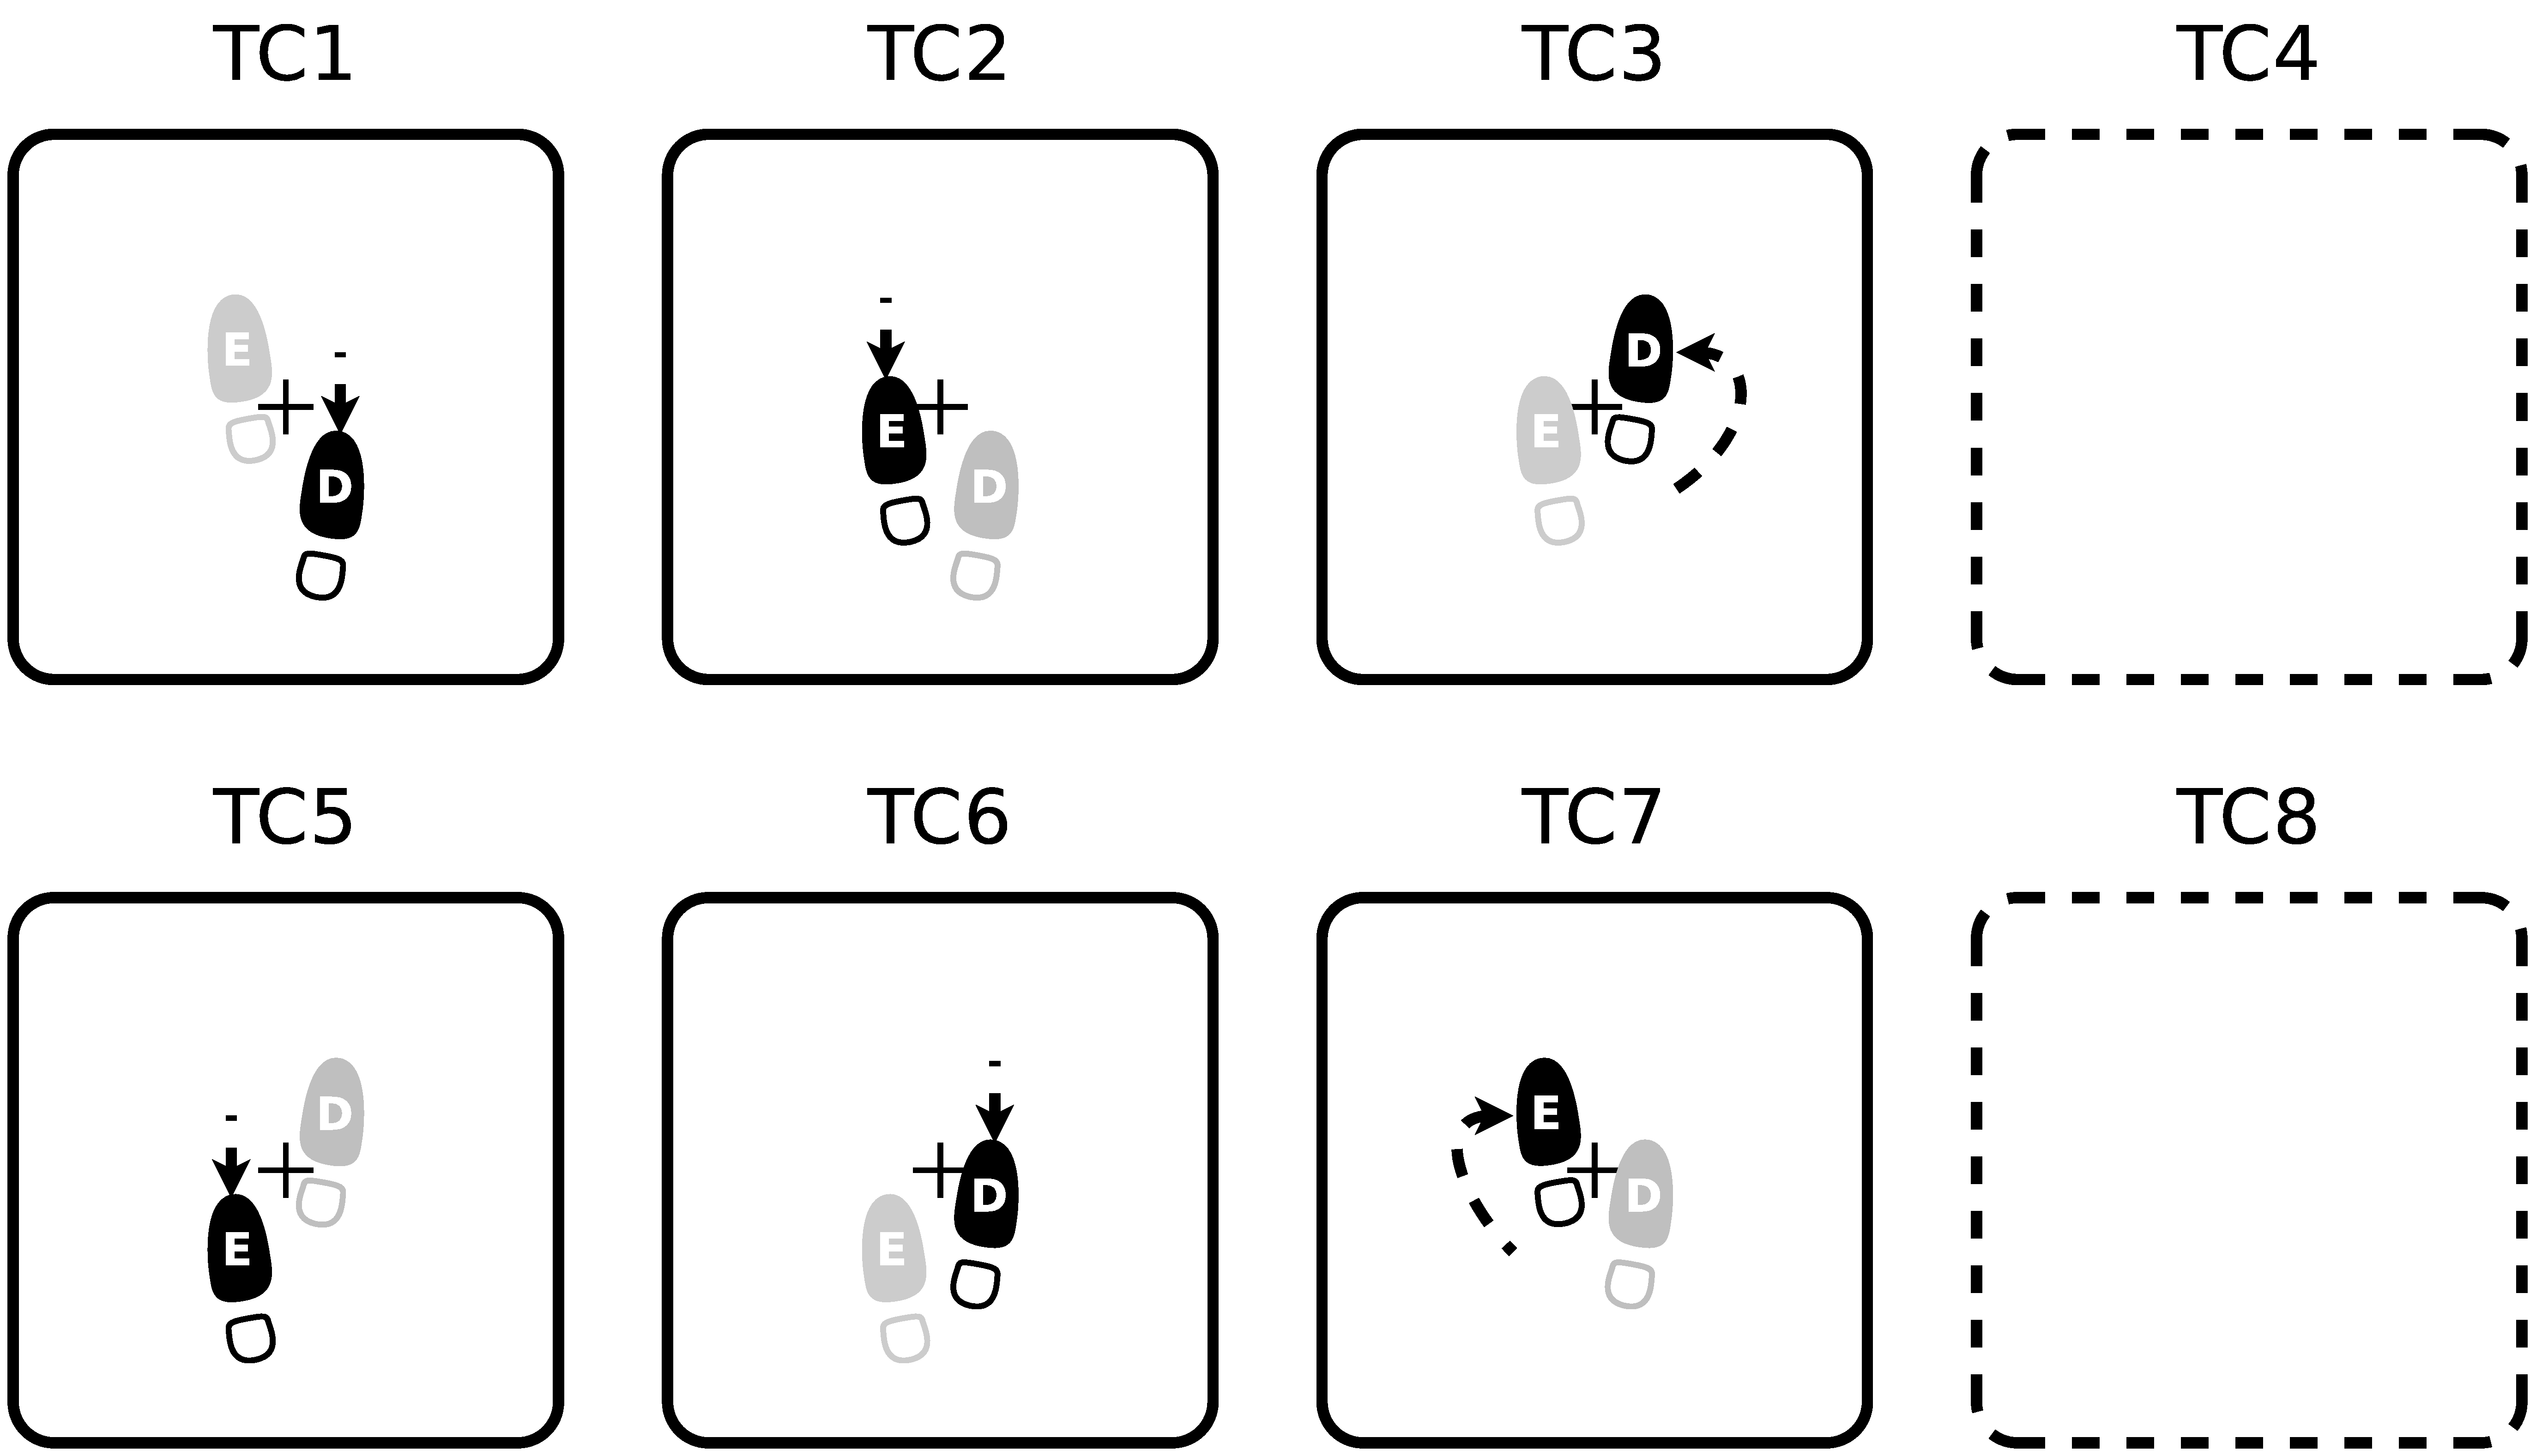
\includegraphics[width=0.75\textwidth]{chapters/cap-passos-footwork/samba-no-pe-adiante.eps}
\caption{Diagrama de tempos coreográficos para o passo de samba no pé para adiante, $T/2=TC$.}
\label{fig:pessoa-samba-no-pe-adiante}
\end{figure}


\subsection{\textcolor{red}{\Variante~2: Samba no pé (para adiante)}}\index{Passo!Samba no pé para adiante}
A Figura \ref{fig:pessoa-samba-no-pe-adiante-b} mostra o diagrama de tempos para realizar o movimento.

\begin{figure}[h]
  \centering
    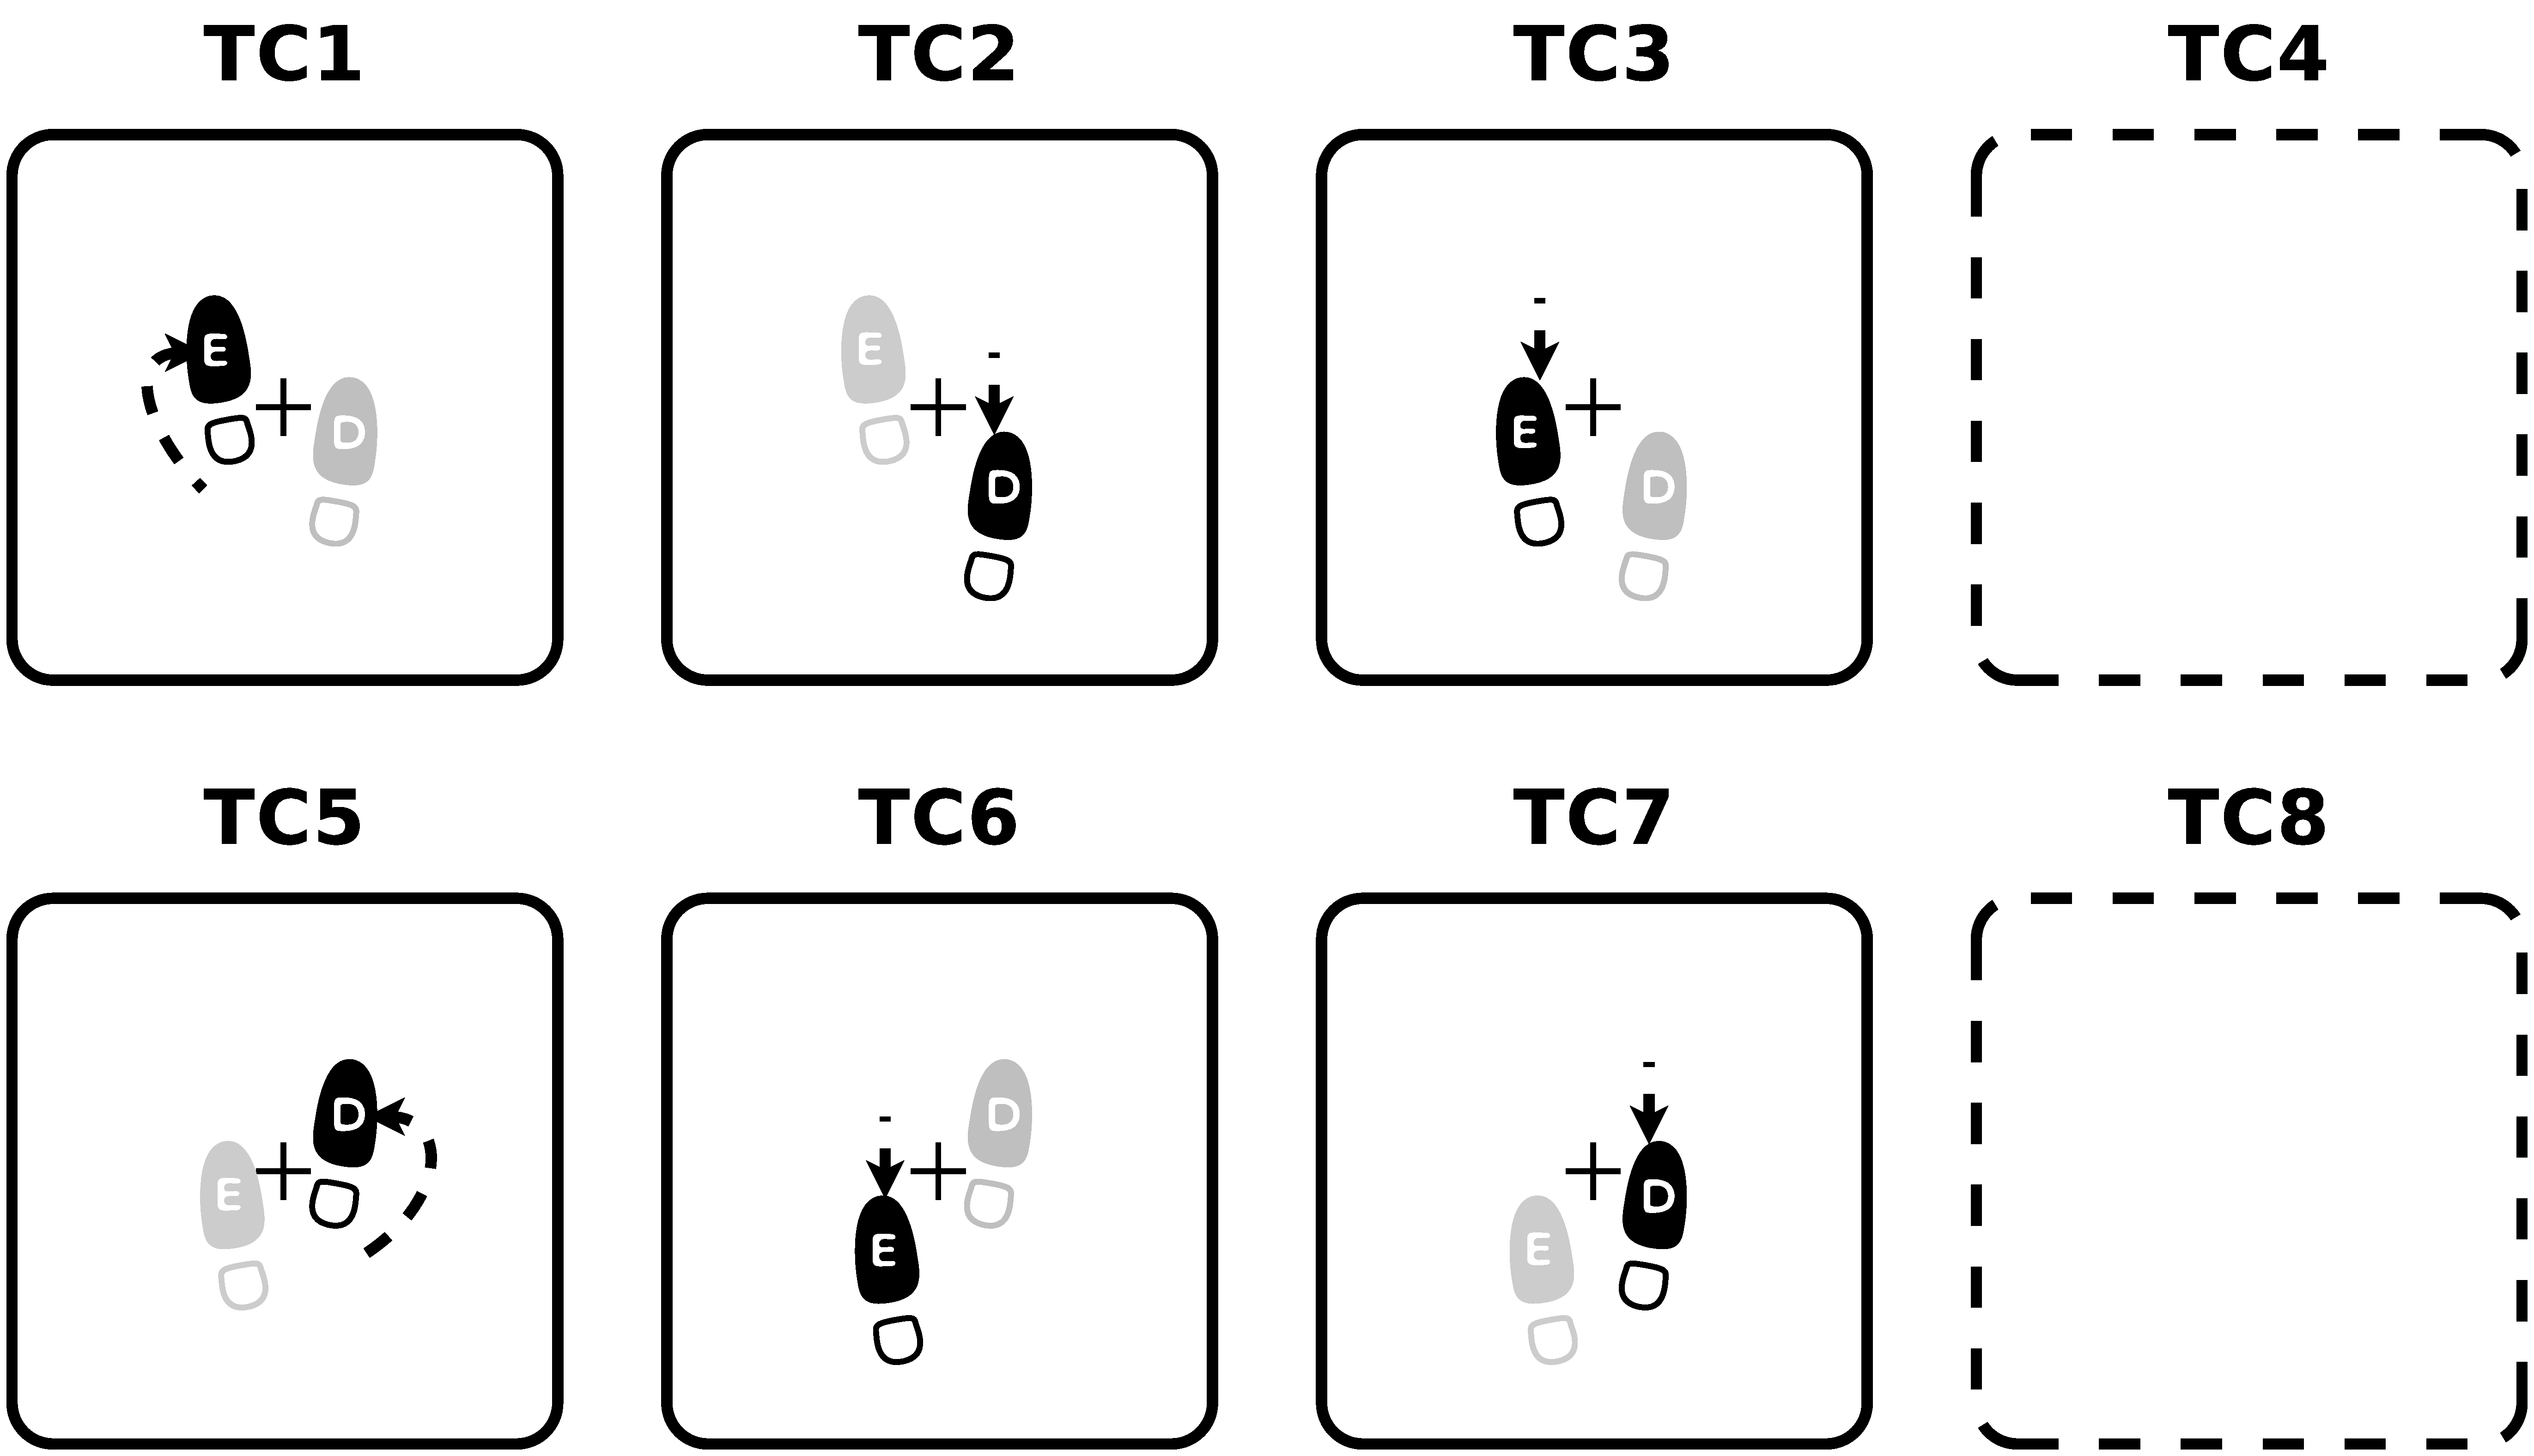
\includegraphics[width=0.75\textwidth]{chapters/cap-passos-footwork/samba-no-pe-adiante-b.eps}
\caption{Diagrama de tempos coreográficos para o passo de samba no pé para adiante, $T/2=TC$.}
\label{fig:pessoa-samba-no-pe-adiante-b}
\end{figure}


\subsection{\textcolor{red}{\Variante: Escovinha (para adiante)}}\index{Passo!Escovinha pra adiante}

A Figura \ref{fig:pessoalescovinha} mostra o diagrama de tempos para realizar o movimento.

\begin{figure}[h]
  \centering
    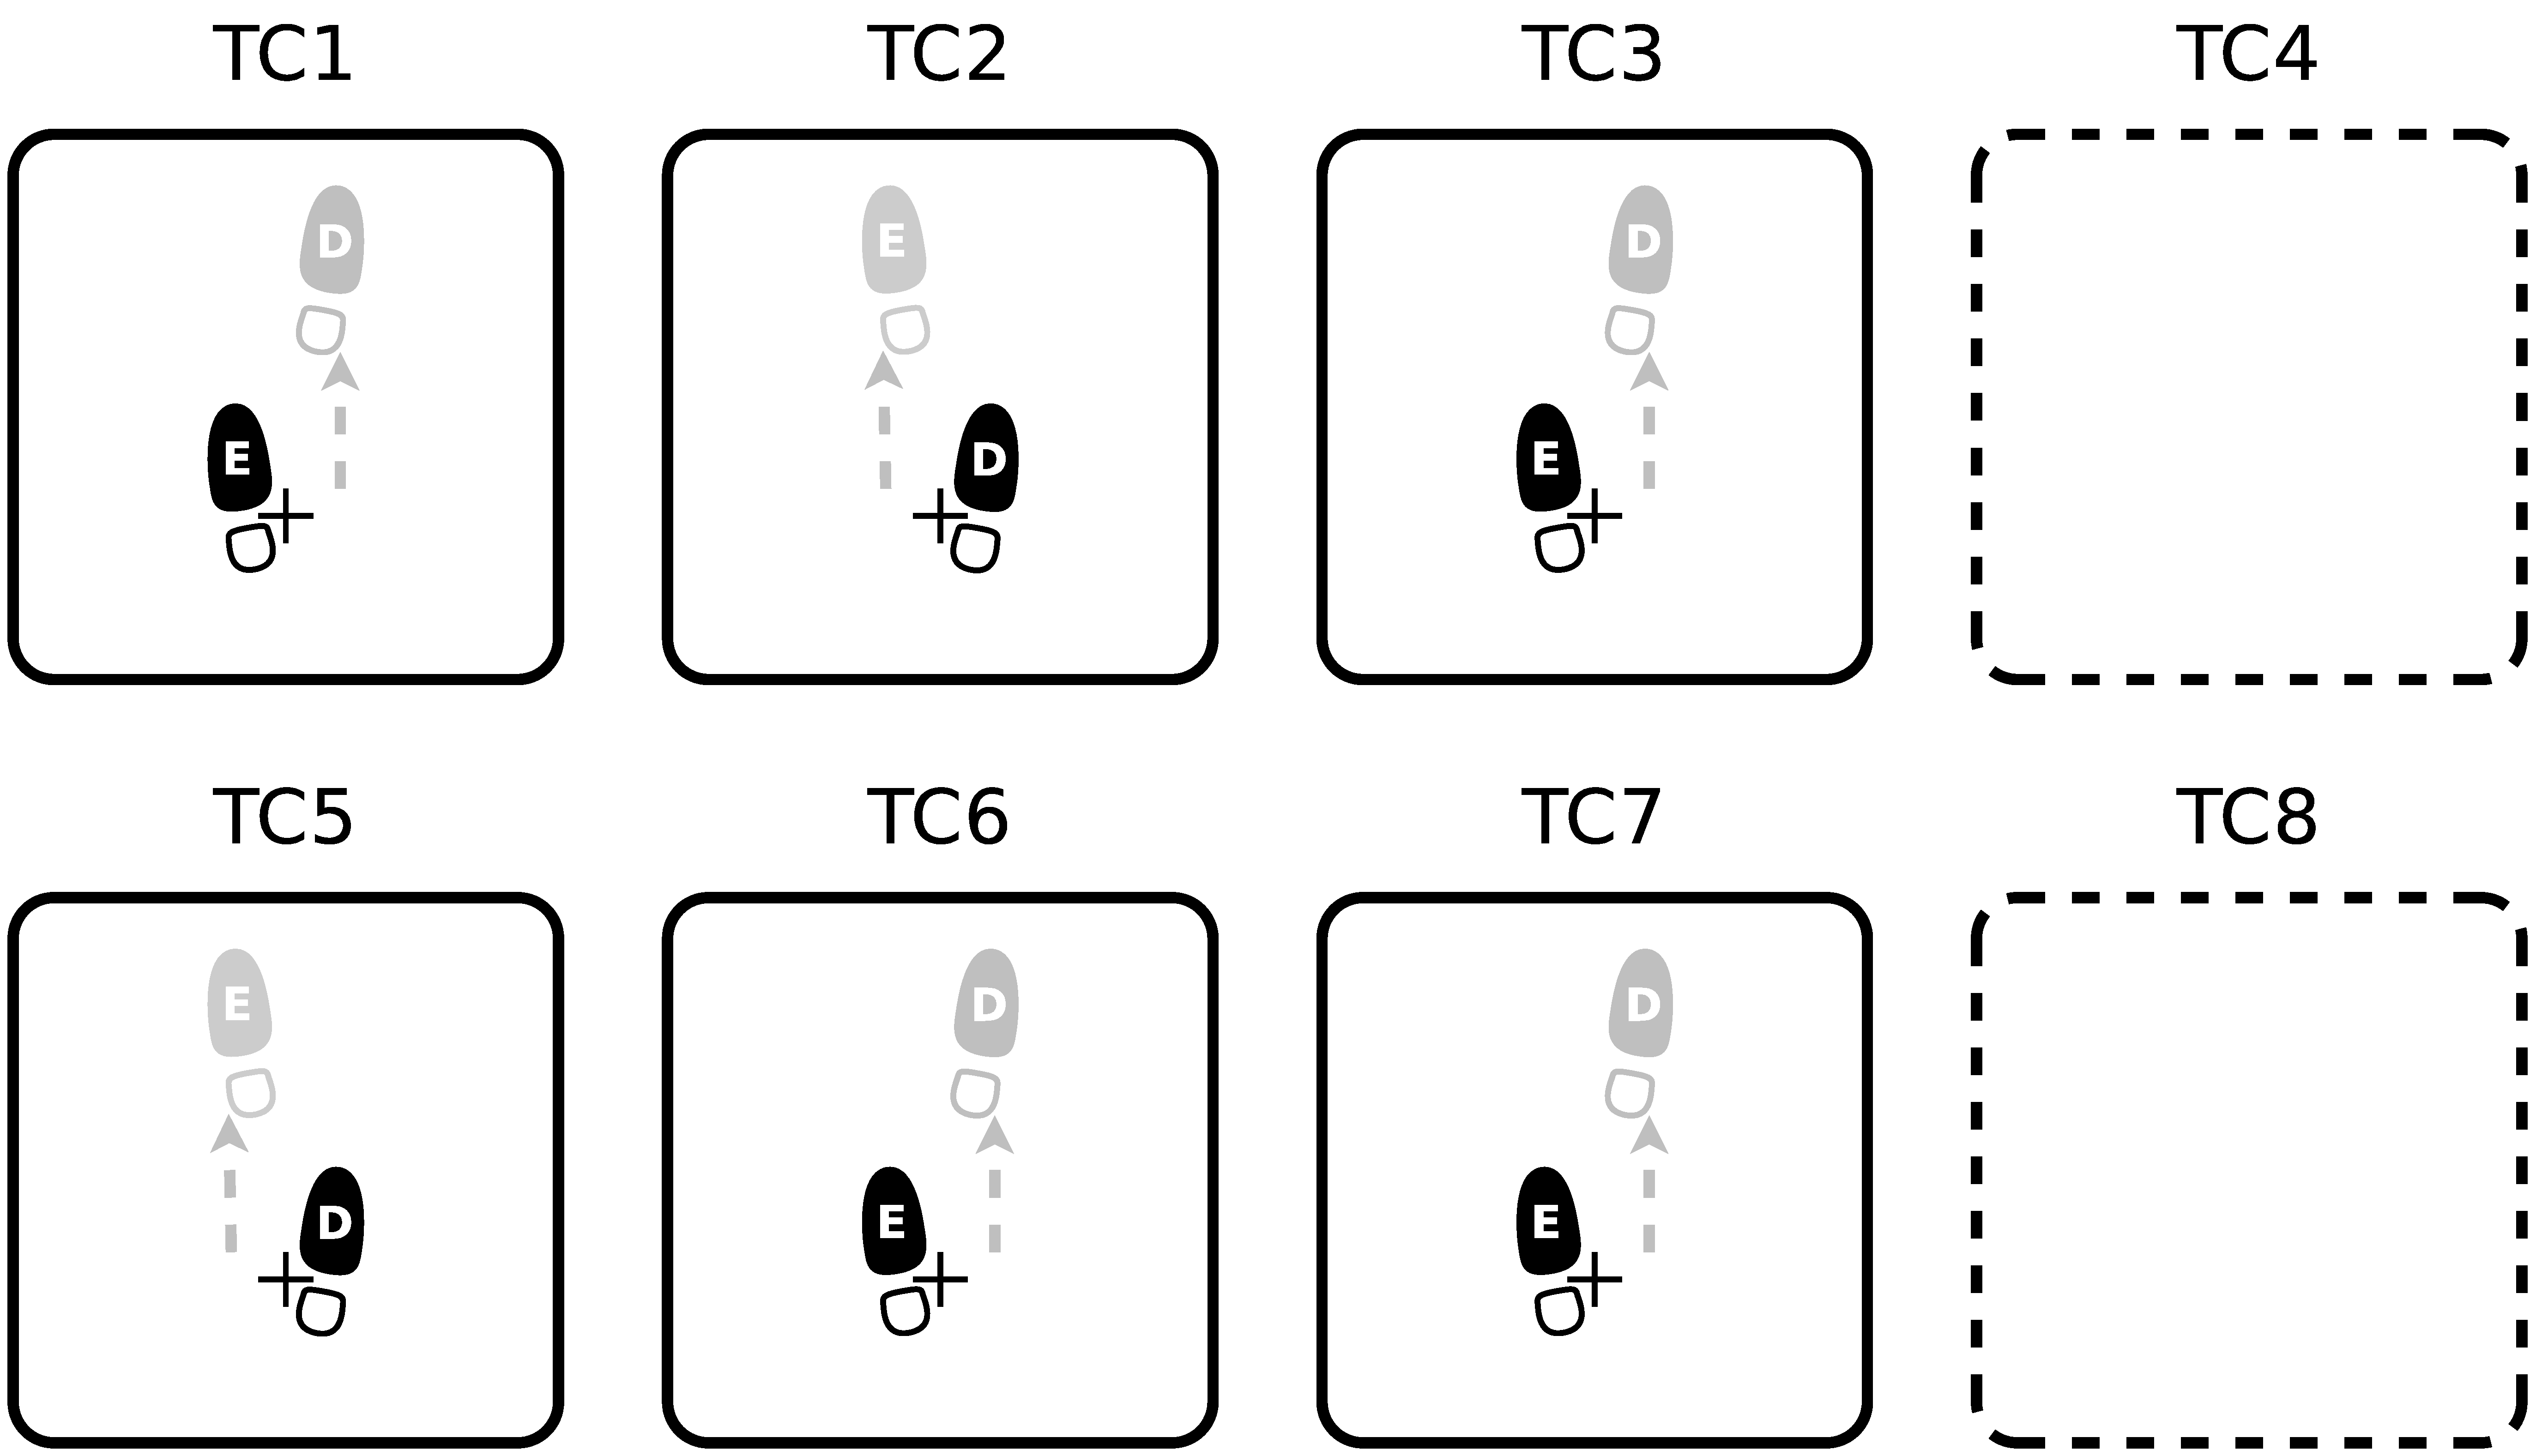
\includegraphics[width=0.75\textwidth]{chapters/cap-passos-footwork/escovinha.eps}
\caption{Diagrama de tempos coreográficos para a escovinha, $T/2=TC$.}
\label{fig:pessoalescovinha}
\end{figure}

A Figura \ref{fig:pessoalescovinha2} mostra o diagrama de tempos para realizar o movimento.
\begin{figure}[h]
  \centering
    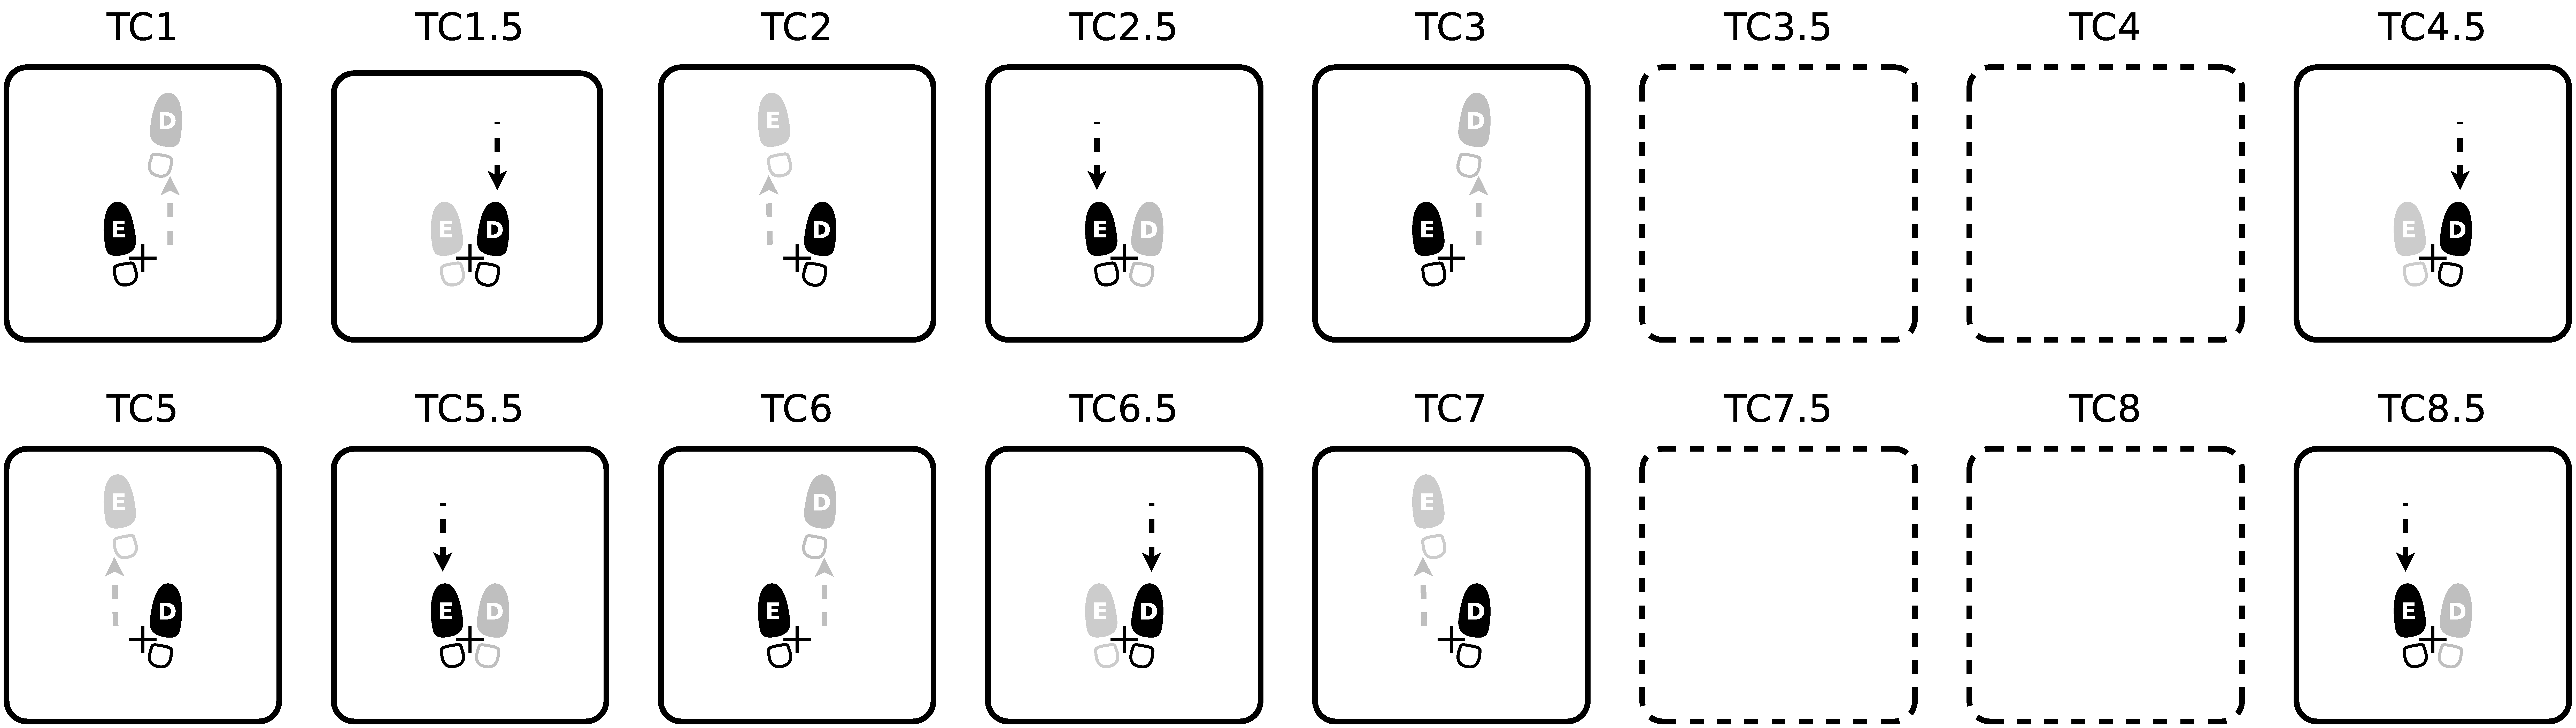
\includegraphics[width=\textwidth]{chapters/cap-passos-footwork/escovinha2.eps}
\caption{Diagrama detalhado de tempos coreográficos para a escovinha, $T/2=TC$.}
\label{fig:pessoalescovinha2}
\end{figure}

\subsection{\textcolor{red}{\Variante: Escovinha (para trás)}}\index{Passo!Escovinha pra trás}

\subsection{\textcolor{red}{\Variante: Escovinha trocando de lados}}\index{Passo!Escovinha trocando de lados}

\subsection{\textcolor{red}{\Variante: Pica-pau}}\index{Passo!Pica-pau}

\subsection{\textcolor{red}{\Variante: Pescaria}}\index{Passo!Pescaria}


